\documentclass[12pt,a4paper,oneside]{report}
\usepackage[utf8]{inputenc}
\usepackage[french]{babel}
\usepackage[T1]{fontenc}
\usepackage{amsmath}
\usepackage{amsfonts}
\usepackage{amssymb}
\usepackage{amscd}
\usepackage{makeidx}
\usepackage[pdftex]{graphicx}
\usepackage{times}
\usepackage{setspace}
\usepackage[left=2.5cm,right=2cm,top=2cm,bottom=2cm]{geometry}
\usepackage{url}
\usepackage{listings}
\usepackage{titlesec}
\usepackage[titletoc]{appendix}
\usepackage[nottoc]{tocbibind}
\usepackage{tikz}
\usepackage{pgfplots}
%\usepackage[screen,nopanel]{pdfscreen}
%\usepackage[lenny]{fncychap}
\usepackage{acronym}
\usepackage{multirow}
\usepackage{graphics}
\usepackage{xcolor}
\usepackage[stable]{footmisc}
\usepackage[textfont={it}]{caption}
\usepackage{pgf}
\usepackage{pdfpages}
\usepackage{mathptmx}
% load package algorithm
\usepackage{algorithm}
\usepackage[noend]{algpseudocode}
% define param
\makeatletter
\def\BState{\State\hskip-\ALG@thistlm}
\makeatother



\usepackage{tocloft}


\usepackage{hyperref}
\hypersetup{colorlinks=true, linkcolor=black, citecolor=black, filecolor=black, urlcolor=black, pdftitle={Theorie des graphes et applications}, pdfauthor=Mirza Andriamanamisoa et Rivo Hermann, pdfsubject=graphe algorithme, pdfkeywords=graphe algorithme}

\usepackage{algorithm2e}

\usepackage{algorithmicx}

\usepackage{algorithm}
\usepackage[noend]{algpseudocode}
%\usepackage{algorithmic}

\author{Mirza Andriamanamisoa MAROTSAHA and Rahajason Rivo Hermann}
\title{Theorie des graphes }
\begin{document}
\maketitle
\renewcommand{\contentsname}{Sommaire}
\tableofcontents
\chapter{Théorie des graphes}
\section{Définitions et concept fondamental (graphe non orienté)}
\subsection{Définitions}
\noindent De façon conceptuelle, un graphe est formé par des sommets (Vertices en anglais) et des arêtes (Edges en anglais) 
qui relient les sommets entre-eux.

\begin{figure}[h]
\centering
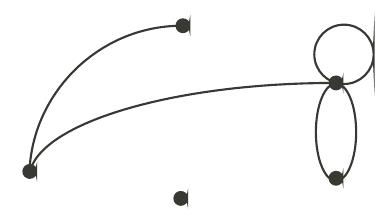
\includegraphics[width=0.5\linewidth]{images/graph}
\caption[Exemple d'un graphe]{Exemple de graphe}
\label{fig:graph}
\end{figure}

\noindent En d'autre terme, un \textbf{graphe} fini noté $G=(V,E)$ est défini par l'ensemble fini $V\ = \{v_{1},\ v_{2},\dots,\ v_{n} \}$ 
dont les éléments sont appelés \textbf{sommets}, 
et par un ensemble fini 
$ E\ = \{ e_{1},\ e_{2},\dots ,\ e_{m} \} $
dont les éléments sont appelés \textbf{arêtes}.

\noindent Une arête $ e $ de l'ensemble $ E $ est définie par une paire non ordonnée de sommets, appelés
les \textbf{extrémités} de $ e $. Si l'arête $ e $ relie les sommets $ u $ et $ v $, on note $ e=\ (u,v) $, on dira que ces sommets sont
\textbf{adjacents}, ou \textbf{incidents} avec $ e $, ou bien que l'arête $ e $ est incidente avec 
les sommets $ u $ et $ v $.\\
Des arêtes sont adjacentes si elle partagent les mêmes extrémités.
On appelle \textbf{ordre} d'un graphe le nombre de sommets n de ce graphe.\\
Les arêtes sont dites \textbf{parallèle} s'ils ont les mêmes extrémités. \\
On appelle \textbf{boucle} l'arête $ e $ de la forme $ (u,u) $. \\
On dit qu'un graphe est un \textbf{graphe simple} s'il ne possède pas des arêtes parallèle et de boucle. \\
Un graphe sans arêtes (c'est-à-dire $E$ est vide )est \textbf{vide}.\\
Un graphe sans sommets (c'est-à-dire $V$ et $E$ sont vides) est un \textbf{graphe nul}.\\
Un graphe avec un seul sommet est dit \textbf{trivial}.\\
Le degré d'un sommet $v$, noté $d(v)$, est le nombre des arêtes qui parent du sommet $v$.
Par convention, une boucle compte deux fois et les arêtes parallèles sont comptées séparément.
Un sommet isolé est un sommet qui a un degré nul.


\begin{figure}[ht]
\centering
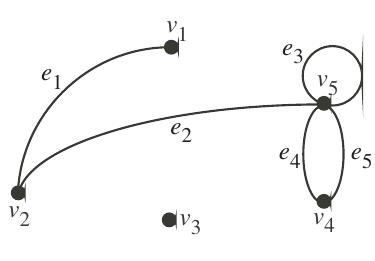
\includegraphics[width=0.5\linewidth]{images/graph1}
\caption[Étiquetage des sommets et des arêtes]{Étiquetage des sommets et des arêtes}
\label{fig:graph1}
\end{figure} 
\paragraph*{}
En prenant l'exemple du Fig. \ref{fig:graph1}:
\begin{itemize}
	\item[\textbullet] $v_{4}$ et $v_{5}$ sont les extrémités de $e_{5}$.
	\item[\textbullet] $e_{4}$ et $e_{5}$ sont parallèle.
	\item[\textbullet] $e_{3}$ est une boucle.
	\item[\textbullet] Ce graphe n'est pas simple.
	\item[\textbullet] $e_{1}$ et $e_{2}$ sont adjacents.
	\item[\textbullet] $v_{1}$ et $v_{2}$ sont adjacentes.
	\item[\textbullet] Le degré du sommet $v_{5}$ est 5.
	\item[\textbullet] Le degré du sommet $v_{4}$ est 2.
	\item[\textbullet] Le degré du sommet $v_{3}$ est 0 donc le sommet est isolé.
\end{itemize}

On note $\delta (G)$ (respectivement $\varDelta (G)$) le degré minimum (respectivement maximum)
des sommets dans le graphe G.
En prenant toujours l'exemple précédent,  $\delta (G) = 0$ et $\varDelta (G) = 5$.
\paragraph*{Remarque.} Dans ce rapport, on considère seulement les graphes finis, c'est-à-dire
$V$ et $E$ sont des ensembles finis.

Comme chaque arêtes ont deux extrémités, on a:

\paragraph*{Théorème 1.1.} Le graphe $G=(V,E)$, où $V = \{v_{1},\dots,v_{n}\}$ et
$E=\{e_{1},\dots,e_{m} \}$, donne
	$$ \sum_{i=1}^{n}d(v_{i})\ =\ 2m  $$
\paragraph*{Corolaire 1.2.} Chaque graphe a un nombre pair de sommets d'un degré impair.

\paragraph*{\textit{Preuve.}} Si les sommets $v_{1},\dots,v_{k}$ ont un degré impair et 
les sommets $v_{k+1},\dots,v_{n}$ ont un degré pair, alors (Théorème 1.1.)
$$ d(v_{1}+\dots +v_{k}=2m -\ d(v_{k+1})\ -\ \dots-d(v_{n})$$ 
est pair. D'où, k pair.

En prenant encore l'exemple précédent, la somme des degrés est $ 1+2+0+2+5 = 10 = 2\times 5$.
Il y a deux sommets d'un degré pair qui sont $v_{1}$ et $v_{5}$.

\paragraph*{}
Un graphe est dit \textit{graphe complet} chaque sommet du graphe est relié directement à tous les autres
sommets.
Un graphe complet avec $n$ sommets est noté $K_{n}$. Les quatre premiers graphes complets sont donnés
par Fig.\ref{fig:graph2}. 

\begin{figure}[h]
\centering
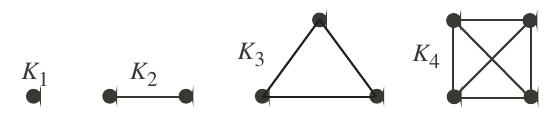
\includegraphics[width=0.5\linewidth]{images/graph2}
\caption[Les quatre premiers graphes complets.]{Les quatre premiers graphes complets.}
\label{fig:graph2}
\end{figure}
\paragraph*{}
\noindent Le graphe $G_{1} = (V_{1},E_{1})$ est un sous-graphe de $G_{2}=(V_{2},E_{2})$ si:
\begin{itemize}
	\item[1.] $V_{1}\subseteq V_{2}$ et
	\item[2.] Chaque arête de $G_{1}$ est aussi une arête de $G_{2}$.
\end{itemize}

\paragraph*{Autres types de graphes}.\\
On appelle \textbf{multigraphes} tous les graphes qui contiennent une boucle, ou
plusieurs arêtes reliant les deux mêmes sommets.

\begin{figure}[h]
\centering
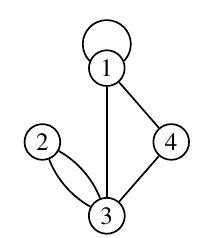
\includegraphics[width=0.2\linewidth]{images/graph3}
\caption[Multigraphe.]{Multigraphe.}
\label{fig:graph3}
\end{figure}

Un graphe est \textbf{connexe} s'il est possible à partir de n'importe quel sommet,
de rejoindre tous les autres en suivant les arêtes. Un graphe non connexe se décompose en composantes
connexes. Sur le graphe ci-dessous, les composantes connexes sont {1, 2, 3, 4} et {5, 6}.
 
\begin{figure}[h]
\centering
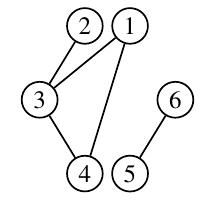
\includegraphics[width=0.2\linewidth]{images/graph4}
\caption[Graphe connexe.]{Graphe connexe.}
\label{fig:graph4}
\end{figure}

Un graphe est \textbf{biparti} si ses sommets peuvent être divisés en deux ensembles X et Y ,
de sorte que toutes les arêtes du graphe relient un sommet dans X à un sommet dans Y
(dans l'exemple ci-dessous, on a X = {1, 3, 5} et Y = {2, 4}, ou vice versa).

\begin{figure}[h]
\centering
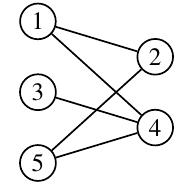
\includegraphics[width=0.2\linewidth]{images/graph5}
\caption[Graphe biparti.]{Graphe biparti.}
\label{fig:graph5}
\end{figure}

\newpage
\subsection{Chaînes et cycles}
\noindent Une \textbf{chaîne} dans G, est une suite ayant pour éléments alternativement des sommets et des
arêtes, commençant et se terminant par un sommet, et telle que chaque arête est encadrée
par ses extrémités.
\paragraph*{}
\noindent On dira que la chaîne \textbf{relie} le premier sommet de la suite au dernier sommet. En plus, on
dira que la chaîne a pour longueur le nombre d'arêtes de la chaîne.

\begin{figure}[h]
\centering
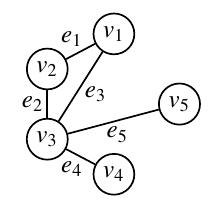
\includegraphics[width=0.2\linewidth]{images/graph6}
\caption[Chaîne.]{Le graphe G contient entre autres les chaînes $ (v_{1} , e_{1} , v_{2} , e_{2} , v_{3} , e_{5} , v_{5} ) $
	et $ (v_{4} , e_{4} , v_{3} , e_{2} , v_{2} , e_{1} , v_{1} ) $.}
\label{fig:graph6}
\end{figure}

\paragraph*{}
\noindent On ne change pas une chaîne en inversant l'ordre des éléments dans la suite correspondante.
Ainsi, les chaînes $ (v_{1} , e_{3} , v_{3} , e_{4} , v_{4} ) $ et
 $ (v_{4} , e_{4} , v_{3} , e_{3} , v_{1} )$ sont identiques.
 
\paragraph*{Théorème 1.3.} Un graphe est biparti si et seulement s’il ne contient aucun cycle de longueur impaire.

\paragraph*{Théorème 1.4.} Pour un graphe $ G $ ayant $ m $ arêtes, $ n $ sommets et $ p $ composantes connexes, on définit :
$$ \nu (G) =m-n+p$$
$ \nu (G) $ est appelé le nombre \textbf{cyclomatique}. Prononcer " nu de G ".
On a $ \nu (G) \geq  0$ pour tout graphe $ G $.
De plus, $ \nu (G) = 0 $ si et seulement si $ G $ est sans cycle.

\subsection{Graphes eulériens}
On appelle \textbf{cycle eulérien} d'un graphe $ G $ un cycle passant une et une seule fois par chacune
des arêtes de $ G $. Un graphe est dit \textbf{eulérien} s'il possède un cycle eulérien.
On appelle \textbf{chaîne eulérienne} d'un graphe G une chaîne passant une et une seule fois par
chacune des arêtes de G. Un graphe ne possédant que des chaînes eulériennes est \textbf{semi-
eulérien}.
Plus simplement, on peut dire qu'un graphe est eulérien (ou semi-eulérien) s'il est possible
de dessiner le graphe sans lever le crayon et sans passer deux fois sur la même arête.

\subsection{Graphes hamiltoniens}
On appelle \textbf{cycle hamiltonien} d'un graphe G un cycle passant une et une seule fois par
chacun des sommets de G. Un graphe est dit \textbf{hamiltonien} s'il possède un cycle hamiltonien.
On appelle \textbf{chaîne hamiltonienne} d'un graphe G une chaîne passant une et une seule fois
par chacun des sommets de G. Un graphe ne possédant que des chaînes hamiltoniennes est
\textbf{semi-hamiltonien}.
Contrairement aux graphes eulériens, il n'existe pas de caractérisation simple des graphes\\
(semi-)hamiltoniens. On peut énoncer quelques propriétés et conditions suffisantes :
\begin{itemize}
	\item un graphe possédant un sommet de degré 1 ne peut pas être hamiltonien ;
	\item si un sommet dans un graphe est de degré 2, alors les deux arêtes incidentes à ce sommet
	doivent faire partie du cycle hamiltonien ;
	\item les graphes complets $ K_{n} $ sont hamiltoniens.
\end{itemize}

\paragraph*{Théorème 1.5.(Ore)} Soit $G$ un graphe simple d'ordre $n\geq 3$. Si pour toute paire $\{x,y\}$ 
de sommets non adjacents, on a $d(x) + d(y) \geq n$, alors $G$ est hamiltonien.

\paragraph*{Corollaire 1.6.(Dirac)} Soit $G$ un graphe simple d'ordre $n\geq 3$. Si pour tout sommet $x$ de $G$,
on a $d(x) \geq \dfrac{n}{2}$, alors $G$ est hamiltonien.

\subsection{Couplages}
Soit $ G $ un graphe simple. Un \textbf{couplage} $ C $ de $ G $ est un sous-graphe partiel 1-régulier de $ G$.
On peut aussi dire qu'un couplage (ou appariement) est un ensemble d'arêtes deux à deux
non-adjacentes.
Un sommet $ v $ est \textbf{saturé} par un couplage $ C $ si $ v $ est l'extrémité d'une arête de $ C $ . Dans le
cas contraire, $ v $ est \textbf{insaturé}.
Un couplage maximum est un couplage contenant le plus grand nombre possible d'arêtes.
Un graphe peut posséder plusieurs couplages maximum.

\begin{figure}[h]
\centering
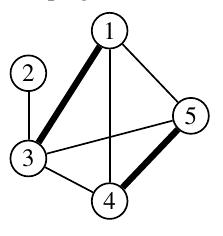
\includegraphics[width=0.3\linewidth]{images/graph8}
\caption{En gras, un couplage maximum de G. Les sommets 1, 3, 4 et 5 sont saturés.}
\label{fig:graph8}
\end{figure}

Un \textbf{couplage parfait} est un couplage où chaque sommet du graphe est saturé.

\begin{figure}[h]
\centering
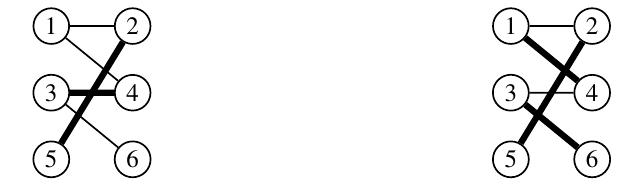
\includegraphics[width=0.7\linewidth]{images/graph9}
\caption{Un couplage (à gauche); Un couplage maximum et parfait (à droite)}
\label{fig:graph9}
\end{figure}

\paragraph*{Calcule d'un couplage maximum }
Si $ C $ est un couplage de $ G $, on appelle \textbf{chaîne alternée} une chaîne élémentaire de \textbf{G} dont
les arêtes sont alternativement dans $ C $ et hors de $ C $.
Une chaîne alternée est dite augmentante si elle relie deux sommets insaturés. Ci-dessus,
à gauche, la chaîne 1-4-3-6 est augmentante. En "intervertissant les épaisseurs" des arêtes
le long de cette chaîne, on obtient un meilleur couplage (ci-dessus, à droite).

\paragraph*{Théorème 1.7.(Berge, 1957)} Un couplage $ C $ est maximum si et seulement 
s'il n'existe pas de chaîne augmentante
relativement à $ C $.


\subsection{Graphes planaires}
On dit qu'un graphe est \textbf{planaire} si on peut le dessiner dans le plan de sorte que ses arêtes
ne se croisent pas. Rappelons que les arêtes ne sont pas forcément rectilignes.
Une \textbf{carte}, ou graphe \textbf{planaire topologique}, est une représentation particulière d'un multigraphe 
planaire fini. On dit qu'une carte est connexe si son graphe l'est. Une carte divise
le plan en plusieurs régions.
Par exemple, la carte ci-dessous, avec sept sommets et neuf arêtes, divise le plan en quatre
régions $(A, B,C, D)$. Trois régions sont limitées alors que la quatrième $(D)$, extérieure au
diagramme, ne l'est pas.

\begin{figure}[h]
\centering
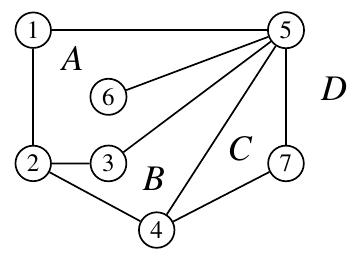
\includegraphics[width=0.4\linewidth]{images/graph10}
\label{fig:graph10}
\end{figure}
\paragraph*{}
\textbf{Le degré d'une région r} , noté $ d(r) $, est la longueur de la chaîne fermée minimum passant 
par tous les sommets qui délimitent cette région. Dans le graphe ci-dessus, $ d(A) = 6 $\\
(la région $ A $ est délimitée par la chaîne fermée passant par les sommets $ (1, 2, 3, 5, 6, 5, 1) $),
$ d(B) = 4 $, $ d(C) = 3 $ et $ d(D) = 5 $.
On remarque que toute arête limite deux régions, ou est contenue dans une région et est
alors comptée deux fois dans la chaîne fermée. Nous avons donc un lemme pour les régions,
analogue au lemme des poignées de mains pour les sommets.

\paragraph*{Théorème 1.8.} La somme des degrés des régions d'une carte connexe est 
égale à deux fois le nombre d'arêtes.

\paragraph*{Théorème 1.9.(Euler 1752)}
Euler a établi une formule célèbre qui relie le nombre de sommets $ S $, le nombre
d'arêtes $ A $ et le nombre de régions $ R $ d'une carte connexe:
$$ S-A+R=2 $$

\paragraph*{Théorème 1.10 (Kuratowski, 1930)}Un graphe est non planaire si et seulement s'il contient 
un sous-graphe homéomorphe (voir lexique) au graphe biparti $ K_{3,3} $ ou au graphe complet $ K_{5} $.

\begin{figure}[h]
\centering
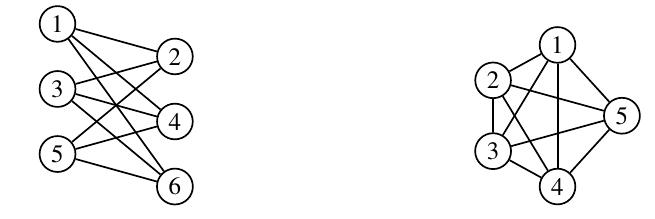
\includegraphics[width=0.7\linewidth]{images/graph11}
\label{fig:graph11}
\end{figure}

\newpage
\subsection{Représentations non graphiques d'un graphe}
\subsubsection{Matrice d'adjacents}
\noindent On peut représenter un graphe simple par une matrice d'adjacences. Une matrice $ (n\times m) $
est un tableau de $ n $ lignes et $ m$  $ $ colonnes. $(i, j)$ désigne l'intersection de la ligne $ i$ et de
la colonne j. Dans une matrice d'adjacences, les lignes et les colonnes représentent les
sommets du graphe. Un $ "1" $  $ $ à la position $ (i, j) $ signifie que le sommet $ i $ est adjacent au
sommet $ j $.

\begin{figure}[h]
\centering
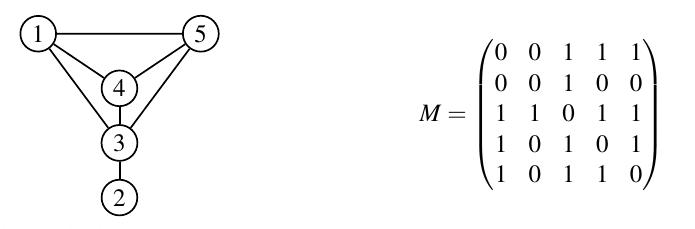
\includegraphics[width=0.7\linewidth]{images/graph7}
\caption[Exemple d'un graphe (à gauche) et sont matrice d'adjacents (à droite).]{Exemple d'un graphe (à gauche) et sont matrice d'adjacents (à droite).}
\label{fig:graph7}
\end{figure}
\paragraph*{}
Cette matrice a plusieurs caractéristiques :

\begin{itemize}
	\item[1.] Elle est carrée : il y a autant de lignes que de colonnes.
	\item[2.] Il n'y a que des zéros sur la diagonale allant du coin supérieur gauche au coin inférieur droit. 
	Un $ "1" $ sur la diagonale indiquerait une boucle.
	\item[3.] Elle est symétrique : $ m_{i j} = m_{ ji} $ . On peut dire que la diagonale est un axe de symétrie.
	\item[4.] Une fois que l'on fixe l'ordre des sommets, il existe une matrice d'adjacences unique
pour chaque graphe. Celle-ci n'est la matrice d'adjacences d'aucun autre graphe.
\end{itemize}
\newpage
\subsubsection{Listes d’adjacences}
\noindent On peut aussi représenter un graphe simple en donnant pour chacun de ses sommets la liste
des sommets auxquels il est adjacent. Ce sont les $ listes d'adjacences $.

\begin{figure}[h]
\centering
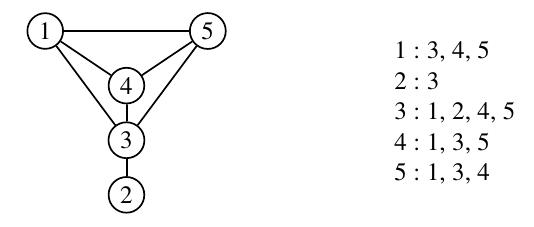
\includegraphics[width=0.7\linewidth]{images/graph12}
\label{fig:graph12}
\end{figure}


\subsection{Arbres}
On appelle \textbf{arbre} tout graphe connexe sans cycle. Un graphe sans cycle mais non connexe
est appelé une \textbf{forêt}.
Une \textbf{feuille} ou \textbf{sommet pendant} est un sommet de degré 1.

\begin{figure}[h]
\centering
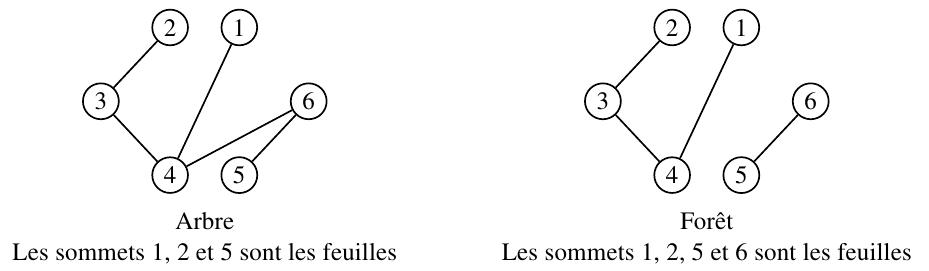
\includegraphics[width=0.7\linewidth]{images/graph13}
\label{fig:graph13}
\end{figure}

\paragraph*{Théorème 1.11.}
Les affirmations suivantes sont équivalentes pour tout graphe G à n sommets.
\begin{itemize}
	\item[1.] $ G $ est un arbre,
	\item[2.] $ G $ est sans cycle et connexe,
	\item[3.] $ G $ est sans cycle et comporte $ n - 1 $ arêtes,
	\item[4.] $ G $ est connexe et comporte $ n - 1 $ arêtes,
	\item[5.] chaque paire $ u,\ v $ de sommets distincts est reliée par une seule chaîne simple (et
	le graphe est sans boucle).
\end{itemize}

\paragraph*{Théorème 1.12.}
Tout arbre fini avec au moins deux sommets comporte au moins deux sommets
pendants.

\subsubsection*{Codage de Prüfer\\}
Le codage de Prüfer (1918) est une manière très compacte de décrire un arbre. Il a été
proposé par le mathématicien allemand Ernst Paul Heinz Prüfer (1896-1934).

\subsubsection*{Codage\\}
Soit l'arbre $ T = (V, E) $ et supposons $ V = \{1, 2, . . . , n \}. $
L'algorithme ci-dessous fournira le code de $ T $ , c'est-à-dire une suite $ S $ de $ n - 2 $ termes
employant (éventuellement plusieurs fois) des nombres choisis parmi $ 1,\dots , n $.
\subsubsection*{Pas général de l'algorithme de codage}
(à répéter tant qu'il reste plus de deux sommets dans l'arbre $ T $ )

\begin{itemize}
	\item[1.] identifier la feuille $ v $ de l'arbre ayant le numéro minimum ;
	\item[2.] ajouter à la suite $ S $ le seul sommet s adjacent à v dans l'arbre $ T $ ;
	\item[3.] enlever de l'arbre $ T $ le sommet $ v $ et l'arête incidente à $ v $.
\end{itemize}

\subsubsection*{Exemple de codage}
\begin{figure}[h]
\centering
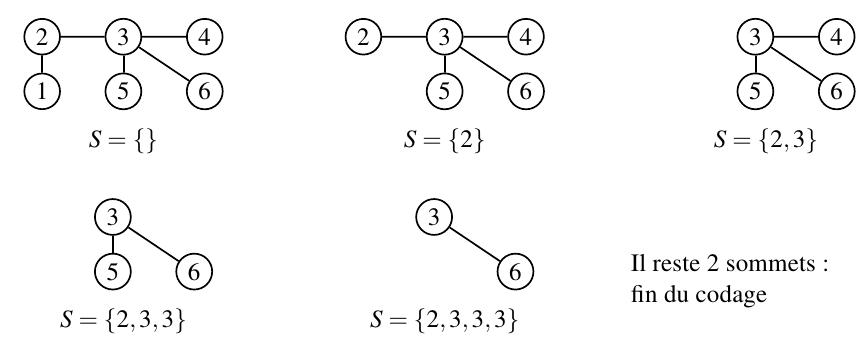
\includegraphics[width=\linewidth]{images/graph14}
\end{figure}

\subsubsection*{Décodage}
Donnée : suite $ S $ de $ n - 2 $ nombres, chacun provenant de $ \{1, \dots , n\} $.
Posons $ I = \{1, \dots , n\} $.
\subsubsection*{Pas général de l'algorithme de décodage}
(à répéter tant qu'il reste des éléments dans $ S $ et plus de deux éléments dans $ I $ )
\begin{itemize}
	\item[1.] identifier le plus petit élément $ i $ de $ I $ n'apparaissant pas dans la suite $ S $ ;
	\item[2.] relier par une arête de $ T $ le sommet $ i $ avec le sommet $ s $ correspondant au premier
élément de la suite $ S $ ;
	\item[3.] enlever $ i $ de $ I $ et $ s $ de $ S $.
\end{itemize}
Les deux éléments qui restent dans $ I $ à la fin de l'algorithme constituent les extrémités de
la dernière arête à ajouter à $ T $ .
\newpage
\subsubsection*{Exemple de décodage}
\begin{figure}[h]
\centering
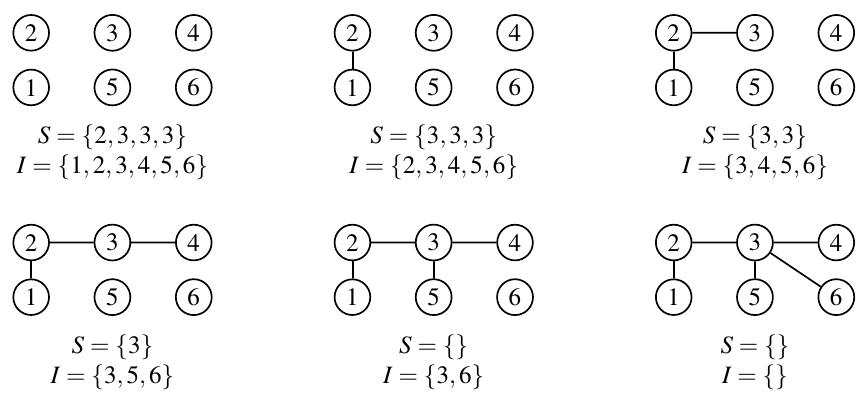
\includegraphics[width=1\linewidth]{images/graph15}
\end{figure}

\paragraph*{Théorème 1.13 (Cayley, 1857)}
Le nombre d'arbres que l'on peut construire sur $ n $ $ (n \geq 2) $ sommets numérotés est
égal à $ n^{n-2} $.

\subsection{Arbres couvrants}
Un \textbf{arbre couvrant} (aussi appelé arbre maximal) est un graphe partiel qui est aussi un
arbre.

\begin{figure}[h]
\centering
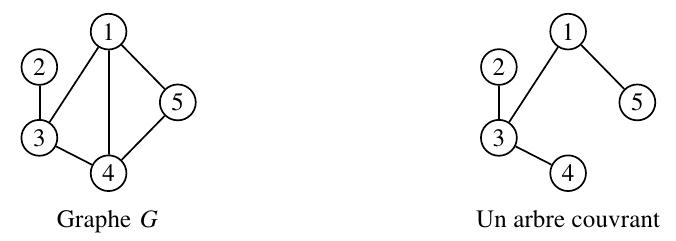
\includegraphics[width=0.7\linewidth]{images/graph16}
\end{figure}

\subsubsection{Arbre couvrant de poids minimum}
Soit le graphe $ G = (V, E) $ avec un poids associé à chacune de ses arêtes. On veut trouver,
dans $ G $, un arbre maximal $ A = (V, F) $ de poids total minimum.

\subsubsection*{Algorithme de Kruskal (1956)}
Données :
\begin{itemize}
	\item Graphe $ G = (V, E) (\textbar V \textbar = n, \textbar E \textbar = m) $
	\item Pour chaque arête e de $ E $ , son poids $ c(e) $.
\end{itemize}
\textit{Résultat} : Arbre ou forêt maximale A = (V, F) de poids minimum.

Trier et renuméroter les arêtes de $ G $ dans l'ordre croissant de leur poids :
$ c(e_{1} ) \leq c(e_{2} ) \leq \dots \leq c(e_{m}) $.
%\begin{algorithm}
%
%\state Poser $ F := \varnothing, k := 0 $
%Tant que $ k < m $ et $ \textbar F\textbar < n - 1 $ faire
%Début
%si $ e_{k}+1 $ ne forme pas de cycle avec $ F $ alors $ F := F \bigcup {e_{k+1} } $
%$ k := k + 1 $
%Fin
%
%\end{algorithm}

\begin{algorithm}
	\caption{Algorithme de Kruskal}\label{euclid}
	\begin{algorithmic}[1]
		\Procedure{}{}
		\State Poser $ F := \varnothing, k := 0 $
		\While {$ k < m $ et $ \textbar F\textbar < n - 1 $}
		\If {$ e_{k}+1 $ ne forme pas de cycle avec $ F $}
		\State$ F := F \bigcup {e_{k+1} } $;
		\EndIf 
		\State $k := k + 1 $;
		\EndWhile
		\EndProcedure
	\end{algorithmic}
\end{algorithm}

\section{Graphe orienté}
\subsection{Définition}

\subsection{Arbres orienté}

\subsection{Graphe orienté acyclique}




\chapter{Theorie des graphes et algorithmes}

\chapter{Applications}


\end{document}